\documentclass[tikz]{standalone}
\usepackage{xcolor}
\definecolor{bg}{HTML}{171D2B}
\definecolor{acc}{HTML}{F7B538}
\definecolor{face}{HTML}{2A3550}
\begin{document}
\pagecolor{bg}
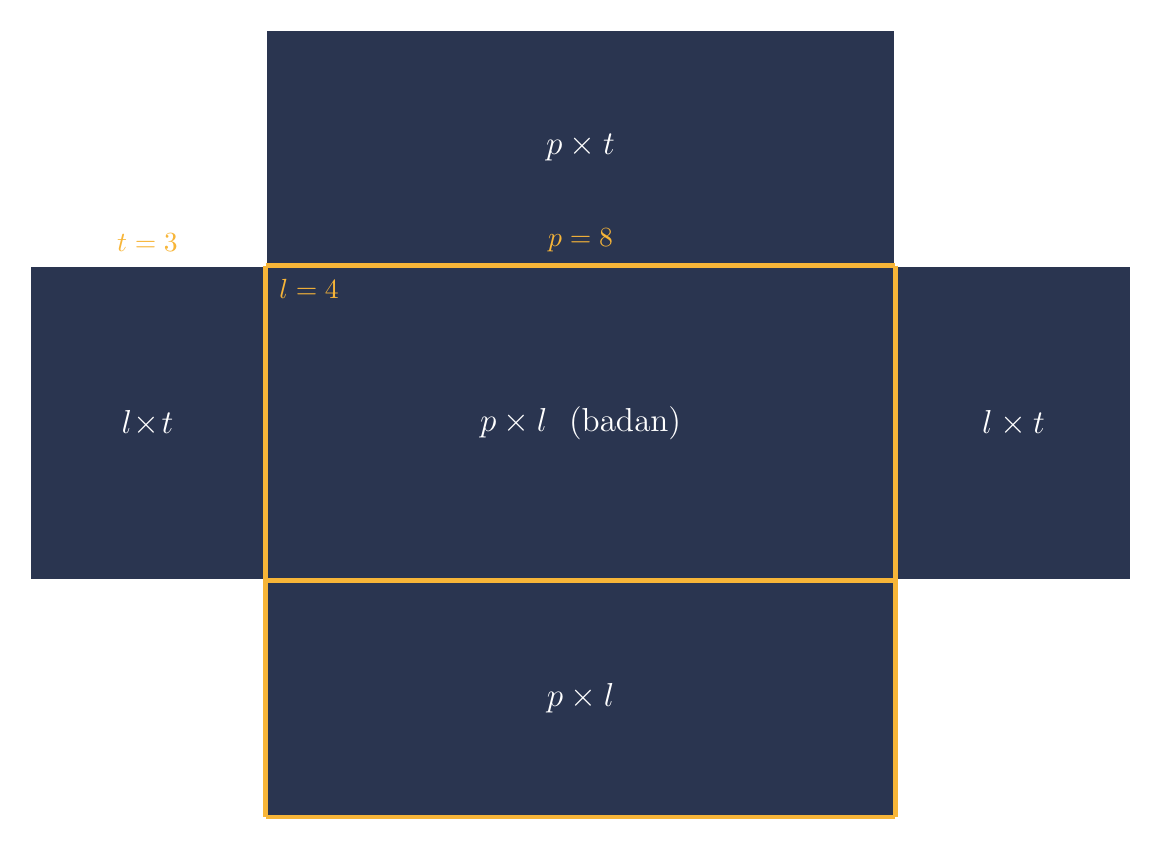
\begin{tikzpicture}[scale=1.0]
  % Jaring-jaring balok: p x l x t = 8 x 4 x 3 (cm)
  % alas di tengah; sisi tegak atas/bawah tinggi t; flap kiri/kanan lebar t
  \def\p{8} \def\l{4} \def\t{3}
  % sisi atas (tutup balok)
  \fill[face,draw=white,line width=1.2pt] (0,0) rectangle (\p,\t);
  \node[white] at (\p/2,\t/2) {\large $p \times t$};
  % sisi bawah (alas)
  \fill[face,draw=white,line width=1.2pt] (0,-\l-\t) rectangle (\p,-\l);
  \node[white] at (\p/2,-\l-\t/2) {\large $p \times l$};
  % sisi tengah (badan): lebar l, tinggi p -> dirotasi: sisi memanjang ke bawah
  \fill[face,draw=white,line width=1.2pt] (0,-\l) rectangle (\p,0);
  \node[white] at (\p/2,-\l/2) {\large $p \times l$ \ (badan)};
  % flap kiri dan kanan (sisi p x t dirotasi)
  \fill[face,draw=white,line width=1.2pt] (-\t,-\l) rectangle (0,0);
  \node[white] at (-\t/2,-\l/2) {\large $l \!\times\! t$};
  \fill[face,draw=white,line width=1.2pt] (\p,-\l) rectangle (\p+\t,0);
  \node[white] at (\p+\t/2,-\l/2) {\large $l \times t$};
  % garis lipat (akses kuning)
  \draw[acc,line width=1.6pt] (0,0) -- (\p,0);
  \draw[acc,line width=1.6pt] (0,-\l) -- (\p,-\l);
  \draw[acc,line width=1.6pt] (0,-\l-\t) -- (\p,-\l-\t);
  \draw[acc,line width=1.6pt] (0,0) -- (0,-\l-\t);
  \draw[acc,line width=1.6pt] (\p,0) -- (\p,-\l-\t);
  % label dimensi
  \node[acc,above] at (\p/2,0.05) {$p=8$};
  \node[acc,below right] at (0.05,-0.05) {$l=4$};
  \node[acc,above] at (-\t/2,0.05) {$t=3$};
\end{tikzpicture}
\end{document}